\documentclass{article}
\usepackage[brazilian]{babel}
\usepackage[utf8]{inputenc}
\usepackage[T1]{fontenc}
\usepackage{graphicx}
\graphicspath{ {./tabelas/} }

\author{Renê Cardozo \\ 
        rene.cardozo@usp.br}

\date{}

\title{Profiling Resource Usage for Mobile Applications \\
        A Cross-layer Approach}

\begin{document}
\maketitle

A criação de aplicações para dispositivos móveis possui características de complexidade intrínseca muitas vezes não
trabalhadas pelos seus desenvolvedores, como a utilização de rede e consumo de energia, geradas diretamente pelas
limitações em recursos destas plataformas.

Pandora, um serviço popular de streaming de música, utilizou cerca de 46\% da sua energia para transmissão de ondas de
rádio em apenas 0.2\% dos dados enviados, devido a uma política de envio de dados contínuos a respeito da sua audiência
de uma maneira mal otimizada.

A ferramenta ARO (Application Resource Optimizer) foi desenvolvida para expor fatores de restrição de protocolos de
camadas mais baixas para o desenvolvimento da aplicação e seu comportamento. Em particular, foi dado foco na interação
entre aplicações e a RAN (Radio Access Network).

ARO é um coletor de dados online e um analisador offline. Primeiramente inicia-se junto a aplicação, capturando dados de
pacotes, sistema e input do usuário; os quais serão direcionados para o software de análise em um computador.

O envio de pequenos pacotes periodicamente (short burst) realizado pelas aplicações é um dos maiores responsáveis pelo
mal uso dos recursos energéticos voltados a radio nos dispositivos móveis. ARO analisa o comportamento das aplicações
com e sem o envio periódico de dados, buscando encontrar um ponto de otimização para o uso de recursos.

\section{Tecnologias Envolvidas}
Uma rede UMTS consiste de três subsistemas, os aparelhos, UTRAN (UMTS Terrestrial Radio Access Network), e a CN (Core
Network). A UTRAN consiste de dois componentes: os Node-B, estações base, e as RNC (Radio Network Controllers),
responsável por controlar múltiplas Node-Bs.

\begin{figure}[!h]
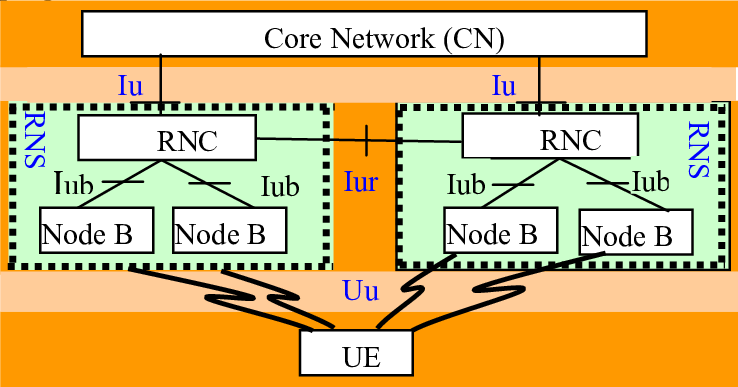
\includegraphics[width=\textwidth]{UTRAN-architecture}
\caption{Arquitetura da rede UTRAM/UMTS relacionando Node-b, RNC e CN}
\centering
\end{figure}

\section{Maquina de Estados}
Nestas redes, o RRC (Radio Resource Control) descreve um autômato finito para cada dispositivo visando o uso eficiente
dos recursos de radio. A máquina de estados é mantida tanto no dispositivo, quanto no RNC (Radio Network Controller), as
quais são sempre sincronizadas por um canal de controle. 

Quando um dispositivo de rede é iniciado seu estado padrão é IDLE, no qual não há nenhuma comunicação com a rede de
controle de radio, sendo a energia consumida próxima de zero. No estado de DCH (Dedicated CHannel) a conexão com a rede é estabelecida e o
dispositivo e será alocado um canal de transporte dedicado para downlink (DL, RNC $\rightarrow$ dispositivo) e para
uplink (UL, dispositivo $\rightarrow$ RNC), permitindo a total utilização dos recursos alocados pelo controle de rede. O
consumo de rede em DCH varia entre 600 a 800 mW por cada antena dos aparelhos celulares ligados à rede UTRAN. O estado FACH (Forward Access CHannel) é intermediário, preservando as conexões estabelecidas
com o controle de recursos, porém somente mantendo um canal de comunicação compartilhado do baixa velocidade. FACH
utiliza pouco mais da metade da energia que o DCH utiliza (55\% até no máximo 75\%).

\subsection{Transição de Estados}
Existem dois tipos de transições de conexão RRC realizadas em uma rede UMTS: promoções, as quais passam de um estado de
baixa energia para mais alta energia; e despromoções, indo na direção reversa. Uma promoção do estado IDLE para um
estado de alta energia ocorre quando qualquer um dos extremos realiza um transferência qualquer de dados. Uma promoção
de FACH para DCH ocorrerá somente quando ocorrer um transferência de dados em alta velocidade, a qual pode ser
detectada pelo uso de uma fila de pacotes em cada ponta da conexão, chamada RLC (Radio Link Controller) buffer. Caso o
tamanho do buffer seja excedido para os pacotes enviados, a conexão é transicionada para o estado DCH. Despromoções são
ativadas por dois temporizadores de inatividade: $\alpha$ (DHC $\rightarrow$ FACH) e $\beta$ (FACH $\rightarrow$ IDLE).

Em cada um dos estados ativos, enquanto são recebidos pacotes o temporizador é posto em um máximo de tempo $T$ e
decrementado após isso. Se nenhum pacote for recebido ou enviado durante esse período $T$, o estado será rebaixado. O
tempo para que um estado permaneça até que seja transferido para um estado de mais baixa energia é chamado de tail time.
Durante este tempo, mesmo transmissões pequenas podem gerar um alto consumo energético se mal administradas.

Cada operadora possui um timer diferente para executar o rebaixamento da conexão, bem como possuem diferentes formas de
transicionar entre estes estados. Uma operadora pode permitir a transição entre IDLE e FACH para poucos dados
transmitidos, enquanto outra irá realizar a promoção de IDLE diretamente para DCH independente da quantidade de dados
iniciais. Além disso, os temporizadores podem ser diferentes para downlink e uplink e variáveis de acordo com a região.

Até o presente momento não existe nenhuma API capaz de informar os estados atuais em que se encontra um aparelho.
Portanto, para efetuar uma análise a partir do dispositivo, é necessário inferir os estados RRC a partir da análise de
pacotes.

\section{Comparando o Consumo de Energia entre LTE e 3G UMTS}
Segundo dados da AT\&T $[1]$, a máquina de estados UMTS tem os seguintes padrões:

\begin{figure}[!h]
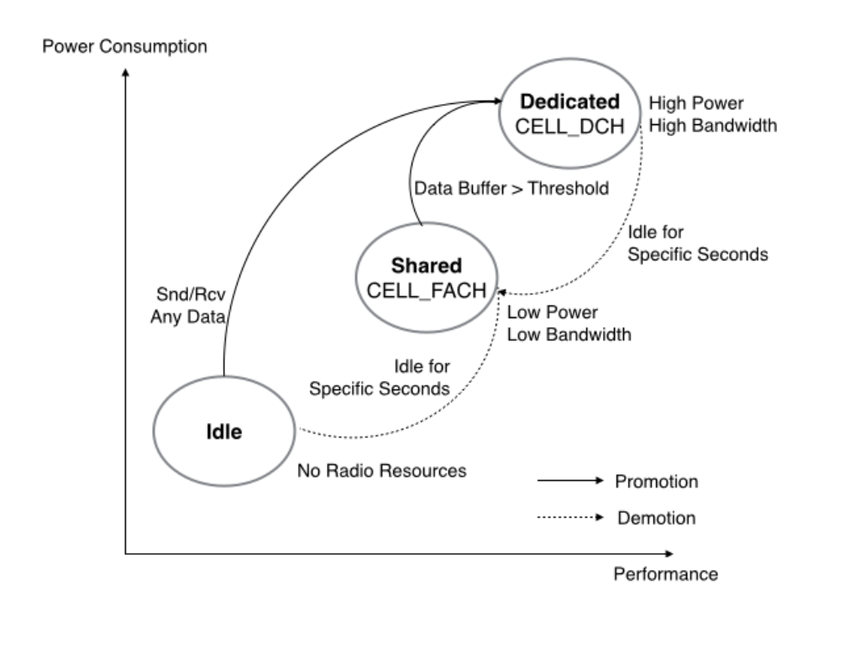
\includegraphics[width=\textwidth]{umts-state-machine}
\caption{Máquina de estados mantida pelo dispositivo e pela RRC}
\centering
\end{figure}

\begin{itemize}
\item IDLE: nenhum consumo energético, sem alocação de banda.
\item CELL\_FACH: baixo consumo energético (460 mW), baixa alocação de banda.
\item CELL\_DCH: alto consumo energético (800 mW), alta alocação de banda.
\end{itemize}

Para redes LTE a máquina de estados opera entre dois estados principais: 
\begin{itemize}
\item RRC\_CONNECTED: radio estará sempre ligado e consumindo entre 1000 e 3500 mW.
\item RRC\_IDLE: radio estará desligado e o consumo de energia será menor do que 15 mW.
\end{itemize}

Enquanto no estado RRC\_CONNECTED o aparelho pode encontrar-se no estado de Continuous Reception, no qual possui alta
capacidade de transferência de dados. Após a transferência ser realizada, o aparelho entrará em Short DRX, no qual o
consumo de energia é mantido alto para esperar a recepção de mais dados, que, caso ocorra, gerará uma promoção para o
estado Continuous Reception novamente. Caso não existam dados durante um período de tempo, o estado será rebaixado para
Long DRX, no qual o dispositivo se prepara para entrar em IDLE (DRX). O aparelho continua em alta energia, escutado a
chegada de pacotes, e, uma vez que cheguem, será promovido diretamente para Continuous Reception. Apenas este último
estado de alta capacidade pode realizar a transferência de dados.


Para redes 3G, a energia utilizada para a transferência de dados em DCH é basicamente constante, independente do
tamanho destes arquivos. Para redes LTE, a energia utilizada pelo estado Continuous Reception varia de acordo com a
banda utilizada. Aparelhos LTE drenam um pouco mais de energia do que aparelhos 3G, uma vez que seus estados
intermediários permanecem em um alto consumo de energia por um longo período para escutar a chegada de pacotes, o que
não ocorre para o 3G, uma vez que possui um estado intermediário FACH que consome metade da energia do DCH.

Apesar de mais rápido, o consumo de energia gerado pelo estado Long DRX do LTE gera um maior consumo de bateria para
redes LTE.

\section{Parâmetros de Inferência}

Para conseguir determinar os estados RRC do dispositivo, existem três principais parâmetros: Os temporizadores de
inatividade; delay para promoção entre estados, que apresenta certa variabilidade há depender da atividade da rede e
operadora; e o tamanho dos buffers RLC, que determina a transição de estados de FACH para DCH, os quais são da ordem de
centenas de bytes e diferentes
para DL e UL, devido a diferenças em seus canais de transporte.

São inclusos parâmetros de ajuste, como: tempo para esvaziamento do buffer RLC, o qual apresenta uma discrepância quanto
a velocidade para downlink (maior) comparada a velocidade de uplink; a não reativação do temporizador de inatividade
para baixas transferências de dados, o que é realizado por algumas operadoras como forma de otimização; e Fast Dormancy,
uma extensão proposta pelo 3GPP para forçar o estado de inatividade antes que os temporizadores expirem, o que diminui o
tail time, porém aumenta o delay para promoção entre estados.

A inferência por pacotes mostra-se mais acurada do que a inferência pela análise energética do aparelho, uma vez que a
última não consegue captar situações de tail time e estão submetidas a um aparelho de medição externo sujeito a ruído.

\section{Descrição de Aplicações Mobile}
Dados em bursts, isto é, transmissões de pequenos pacotes que ocorrem em menos do que $\delta$ segundos, é responsável por
grande parte do consumo de rede e energia destinada a radio dos aparelhos. ARO utiliza um algoritmo para a análise das
causas originárias dos bursts em cada conjunto de dados. Grandes bursts são entendidos como formas eficientes de
transferência de dados, pois oferecem maior aproveitamento do estado de alta energia DCH, Bursts podem ser também
causados pelos pacotes de controle e recuperação de perdas do TCP, bem como por informações menores enviadas pelos
aplicativos com base em temporizadores internos das aplicações. 

\section{Resultados}
Para o serviço de streaming Pandora, o maior consumo de energia foi gerado pelo envio periódico de dados pelo usuário
para os servidores da empresa, os quais contabilizaram 46\% do consumo para 0.2\% os dados. Em comparação, um download
de uma música inteira é realizado em menos de 30 segundos, consumindo menos de 36\% da energia utilizada pela conexão.
Pacotes de controle do TCP foram responsáveis por 1.6\% do consumo energético em seu máximo e 0.6\% para recuperação de
perdas.

\begin{figure}[!h]
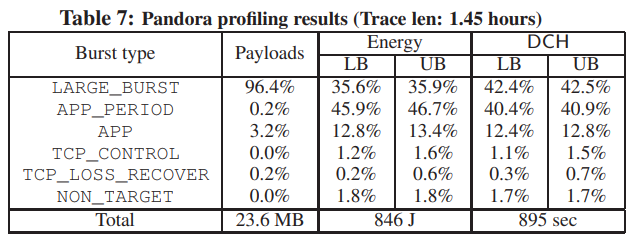
\includegraphics[width=\textwidth]{tabela-pandora}
\caption{UB (upperbound) e LB (lowerbound) referem-se ao maior valor registrado durante todo o intervalo medido.}
\centering
\end{figure}

Para o aplicativo Fox News, a maior parte dos dados foi obtido pelo click ativo dos usuários na tela para acessar
notícias, contudo, apesar de consumir apenas 6\% dos dados totais, as requisições por scroll, alimentadas em maior parte
pelas tumbnails das notícias, consumiram 17.9\% da energia de radio da conexão. Pacote de controle TCP foram responsáveis
por quase 4\% em suas maiores taxas, mesmo representando uma transferência de dados desprezível quando comparada ao
restante dos pacotes. Recuperação de perdas representou 2.5\% da energia utilizada para 1.5\% dos dados em seu maior
uso energético.

\begin{figure}[!h]
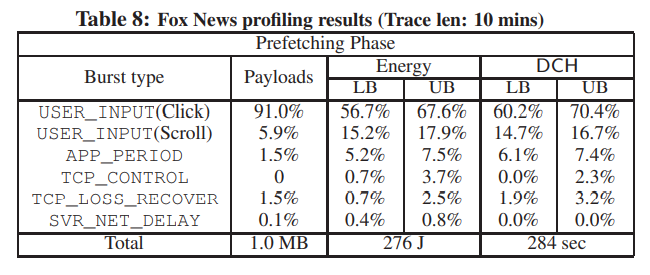
\includegraphics[width=\textwidth]{tabela-fox-news}
\caption{UB (upperbound) e LB (lowerbound) referem-se ao maior valor registrado durante todo o intervalo medido.}
\centering
\end{figure}


O aplicativo BBC News, ao contrário do concorrente, realiza o download de todas as notícias em cache quando uma
determinada categoria é selecionada pelo usuário. Contudo, sua estratégia de uma requisição HTTP para cada notícia gera
uma grande latência, o que poderia ser mitigada através da utilização de HTTP pipelining. Ainda, a demora para o
fechamento das conexões TCP faz com que bursts de FIN e RST sejam disparados, consumindo cerca de 24.2\% da energia
dedicada a radio em seu maior consumo para praticamente nenhuma informação transferida além dos headers do protocolo.
Para determinadas aplicações, como Facebook e Amazon Shopping, as conexões são encerradas logo após os conteúdos das
requisições serem recebidos, contudo, para a BBC News, há um delay de quase 15 segundos em alguns pacotes, e 50\% dos
pacotes FIN/RST são atrasados em 5 segundos, o que gera a promoção de FACH para DCH. Uma estratégia eficiente para
evitar a abertura de novas conexões é realizar o fechamento das conexões antes que o temporizador de promoção de FACH
para DCH seja ativado, uma vez que pacotes pequenos não resetam o temporizador para algumas operadoras.

\begin{figure}[!h]
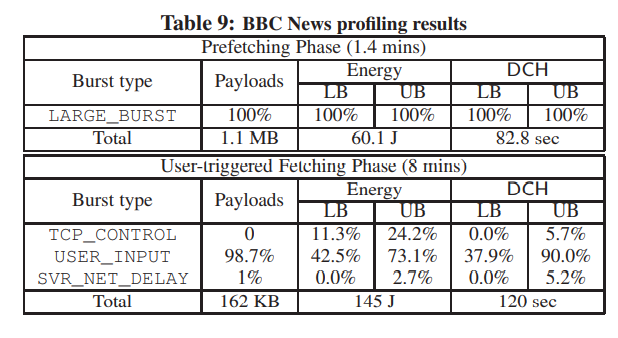
\includegraphics[width=\textwidth]{tabela-bbc-news}
\caption{UB (upperbound) e LB (lowerbound) referem-se ao maior valor registrado durante todo o intervalo medido.}
\centering
\end{figure}


A maior parte da energia consumida para buscas no Google foi causada por queries de sugestões de pesquisa para o
usuário.

SDKs que promovem a adição de anúncios em aplicações consumirão mais energia tanto mais rápido quanto o delay de
atualização de seus anúncios na tela.

\section{Referências}
Artigo Principal: Qian, Feng \& Wang, Zhaoguang \& Gerber, Alexandre \& Mao, Zhuoqing \& Sen, Subhabrata \& Spatscheck,
Oliver. (2011). Profiling Resource Usage for Mobile Applications: a Cross-layer Approach. 321-334.
10.1145/1999995.2000026. \\
1 - Comparing LTE and 3G Energy Consumption -
https://developer.att.com/video-optimizer/docs/best-practices/comparing-lte-and-3g-energy-consumption \\

imagem UTRAN: https://www.researchgate.net/figure/UTRAN-architecture-UMTS-uses-Wideband-Code-Division-Multiple-Access-WCDMA-to-carry-the\_fig1\_228868328

image RRC-state-machine: https://www.researchgate.net/figure/RRC-State-Machine-for-UMTS-Network\_fig1\_299931683

\end{document}

